\documentclass[1p]{elsarticle_modified}
%\bibliographystyle{elsarticle-num}

%\usepackage[colorlinks]{hyperref}
%\usepackage{abbrmath_seonhwa} %\Abb, \Ascr, \Acal ,\Abf, \Afrak
\usepackage{amsfonts}
\usepackage{amssymb}
\usepackage{amsmath}
\usepackage{amsthm}
\usepackage{scalefnt}
\usepackage{amsbsy}
\usepackage{kotex}
\usepackage{caption}
\usepackage{subfig}
\usepackage{color}
\usepackage{graphicx}
\usepackage{xcolor} %% white, black, red, green, blue, cyan, magenta, yellow
\usepackage{float}
\usepackage{setspace}
\usepackage{hyperref}

\usepackage{tikz}
\usetikzlibrary{arrows}

\usepackage{multirow}
\usepackage{array} % fixed length table
\usepackage{hhline}

%%%%%%%%%%%%%%%%%%%%%
\makeatletter
\renewcommand*\env@matrix[1][\arraystretch]{%
	\edef\arraystretch{#1}%
	\hskip -\arraycolsep
	\let\@ifnextchar\new@ifnextchar
	\array{*\c@MaxMatrixCols c}}
\makeatother %https://tex.stackexchange.com/questions/14071/how-can-i-increase-the-line-spacing-in-a-matrix
%%%%%%%%%%%%%%%

\usepackage[normalem]{ulem}

\newcommand{\msout}[1]{\ifmmode\text{\sout{\ensuremath{#1}}}\else\sout{#1}\fi}
%SOURCE: \msout is \stkout macro in https://tex.stackexchange.com/questions/20609/strikeout-in-math-mode

\newcommand{\cancel}[1]{
	\ifmmode
	{\color{red}\msout{#1}}
	\else
	{\color{red}\sout{#1}}
	\fi
}

\newcommand{\add}[1]{
	{\color{blue}\uwave{#1}}
}

\newcommand{\replace}[2]{
	\ifmmode
	{\color{red}\msout{#1}}{\color{blue}\uwave{#2}}
	\else
	{\color{red}\sout{#1}}{\color{blue}\uwave{#2}}
	\fi
}

\newcommand{\Sol}{\mathcal{S}} %segment
\newcommand{\D}{D} %diagram
\newcommand{\A}{\mathcal{A}} %arc


%%%%%%%%%%%%%%%%%%%%%%%%%%%%%5 test

\def\sl{\operatorname{\textup{SL}}(2,\Cbb)}
\def\psl{\operatorname{\textup{PSL}}(2,\Cbb)}
\def\quan{\mkern 1mu \triangleright \mkern 1mu}

\theoremstyle{definition}
\newtheorem{thm}{Theorem}[section]
\newtheorem{prop}[thm]{Proposition}
\newtheorem{lem}[thm]{Lemma}
\newtheorem{ques}[thm]{Question}
\newtheorem{cor}[thm]{Corollary}
\newtheorem{defn}[thm]{Definition}
\newtheorem{exam}[thm]{Example}
\newtheorem{rmk}[thm]{Remark}
\newtheorem{alg}[thm]{Algorithm}

\newcommand{\I}{\sqrt{-1}}
\begin{document}

%\begin{frontmatter}
%
%\title{Boundary parabolic representations of knots up to 8 crossings}
%
%%% Group authors per affiliation:
%\author{Yunhi Cho} 
%\address{Department of Mathematics, University of Seoul, Seoul, Korea}
%\ead{yhcho@uos.ac.kr}
%
%
%\author{Seonhwa Kim} %\fnref{s_kim}}
%\address{Center for Geometry and Physics, Institute for Basic Science, Pohang, 37673, Korea}
%\ead{ryeona17@ibs.re.kr}
%
%\author{Hyuk Kim}
%\address{Department of Mathematical Sciences, Seoul National University, Seoul 08826, Korea}
%\ead{hyukkim@snu.ac.kr}
%
%\author{Seokbeom Yoon}
%\address{Department of Mathematical Sciences, Seoul National University, Seoul, 08826,  Korea}
%\ead{sbyoon15@snu.ac.kr}
%
%\begin{abstract}
%We find all boundary parabolic representation of knots up to 8 crossings.
%
%\end{abstract}
%\begin{keyword}
%    \MSC[2010] 57M25 
%\end{keyword}
%
%\end{frontmatter}

%\linenumbers
%\tableofcontents
%
\newcommand\colored[1]{\textcolor{white}{\rule[-0.35ex]{0.8em}{1.4ex}}\kern-0.8em\color{red} #1}%
%\newcommand\colored[1]{\textcolor{white}{ #1}\kern-2.17ex	\textcolor{white}{ #1}\kern-1.81ex	\textcolor{white}{ #1}\kern-2.15ex\color{red}#1	}

{\Large $\underline{12a_{1199}~(K12a_{1199})}$}

\setlength{\tabcolsep}{10pt}
\renewcommand{\arraystretch}{1.6}
\vspace{1cm}\begin{tabular}{m{100pt}>{\centering\arraybackslash}m{274pt}}
\multirow{5}{120pt}{
	\centering
	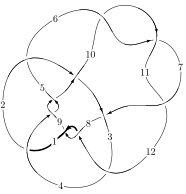
\includegraphics[width=112pt]{../../../GIT/diagram.site/Diagrams/png/2000_12a_1199.png}\\
\ \ \ A knot diagram\footnotemark}&
\allowdisplaybreaks
\textbf{Linearized knot diagam} \\
\cline{2-2}
 &
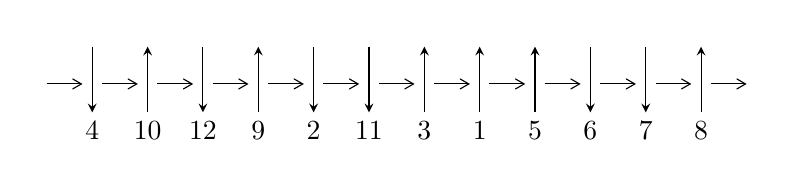
\begin{tikzpicture}[x=20pt, y=17pt]
	% nodes
	\node (C0) at (0, 0) {};
	\node (C1) at (1, 0) {};
	\node (C1U) at (1, +1) {};
	\node (C1D) at (1, -1) {4};

	\node (C2) at (2, 0) {};
	\node (C2U) at (2, +1) {};
	\node (C2D) at (2, -1) {10};

	\node (C3) at (3, 0) {};
	\node (C3U) at (3, +1) {};
	\node (C3D) at (3, -1) {12};

	\node (C4) at (4, 0) {};
	\node (C4U) at (4, +1) {};
	\node (C4D) at (4, -1) {9};

	\node (C5) at (5, 0) {};
	\node (C5U) at (5, +1) {};
	\node (C5D) at (5, -1) {2};

	\node (C6) at (6, 0) {};
	\node (C6U) at (6, +1) {};
	\node (C6D) at (6, -1) {11};

	\node (C7) at (7, 0) {};
	\node (C7U) at (7, +1) {};
	\node (C7D) at (7, -1) {3};

	\node (C8) at (8, 0) {};
	\node (C8U) at (8, +1) {};
	\node (C8D) at (8, -1) {1};

	\node (C9) at (9, 0) {};
	\node (C9U) at (9, +1) {};
	\node (C9D) at (9, -1) {5};

	\node (C10) at (10, 0) {};
	\node (C10U) at (10, +1) {};
	\node (C10D) at (10, -1) {6};

	\node (C11) at (11, 0) {};
	\node (C11U) at (11, +1) {};
	\node (C11D) at (11, -1) {7};

	\node (C12) at (12, 0) {};
	\node (C12U) at (12, +1) {};
	\node (C12D) at (12, -1) {8};
	\node (C13) at (13, 0) {};

	% arrows
	\draw[->,>={angle 60}]
	(C0) edge (C1) (C1) edge (C2) (C2) edge (C3) (C3) edge (C4) (C4) edge (C5) (C5) edge (C6) (C6) edge (C7) (C7) edge (C8) (C8) edge (C9) (C9) edge (C10) (C10) edge (C11) (C11) edge (C12) (C12) edge (C13) ;	\draw[->,>=stealth]
	(C1U) edge (C1D) (C2D) edge (C2U) (C3U) edge (C3D) (C4D) edge (C4U) (C5U) edge (C5D) (C6U) edge (C6D) (C7D) edge (C7U) (C8D) edge (C8U) (C9D) edge (C9U) (C10U) edge (C10D) (C11U) edge (C11D) (C12D) edge (C12U) ;
	\end{tikzpicture} \\
\hhline{~~} \\& 
\textbf{Solving Sequence} \\ \cline{2-2} 
 &
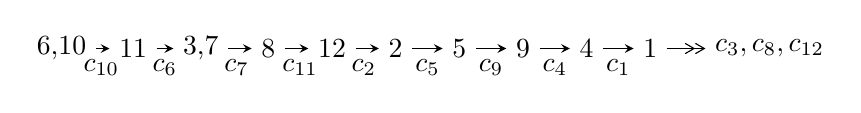
\begin{tikzpicture}[x=23pt, y=7pt]
	% node
	\node (A0) at (-1/8, 0) {6,10};
	\node (A1) at (1, 0) {11};
	\node (A2) at (33/16, 0) {3,7};
	\node (A3) at (25/8, 0) {8};
	\node (A4) at (33/8, 0) {12};
	\node (A5) at (41/8, 0) {2};
	\node (A6) at (49/8, 0) {5};
	\node (A7) at (57/8, 0) {9};
	\node (A8) at (65/8, 0) {4};
	\node (A9) at (73/8, 0) {1};
	\node (C1) at (1/2, -1) {$c_{10}$};
	\node (C2) at (3/2, -1) {$c_{6}$};
	\node (C3) at (21/8, -1) {$c_{7}$};
	\node (C4) at (29/8, -1) {$c_{11}$};
	\node (C5) at (37/8, -1) {$c_{2}$};
	\node (C6) at (45/8, -1) {$c_{5}$};
	\node (C7) at (53/8, -1) {$c_{9}$};
	\node (C8) at (61/8, -1) {$c_{4}$};
	\node (C9) at (69/8, -1) {$c_{1}$};
	\node (A10) at (11, 0) {$c_{3},c_{8},c_{12}$};

	% edge
	\draw[->,>=stealth]	
	(A0) edge (A1) (A1) edge (A2) (A2) edge (A3) (A3) edge (A4) (A4) edge (A5) (A5) edge (A6) (A6) edge (A7) (A7) edge (A8) (A8) edge (A9) ;
	\draw[->>,>={angle 60}]	
	(A9) edge (A10);
\end{tikzpicture} \\ 

\end{tabular} \\

\footnotetext{
The image of knot diagram is generated by the software ``\textbf{Draw programme}" developed by Andrew Bartholomew(\url{http://www.layer8.co.uk/maths/draw/index.htm\#Running-draw}), where we modified some parts for our purpose(\url{https://github.com/CATsTAILs/LinksPainter}).
}\phantom \\ \newline 
\centering \textbf{Ideals for irreducible components\footnotemark of $X_{\text{par}}$} 
 
\begin{align*}
I^u_{1}&=\langle 
-1107 u^{29}-7807 u^{28}+\cdots+74 b-1824,\;609 u^{29}+5328 u^{28}+\cdots+74 a+3095,\\
\phantom{I^u_{1}}&\phantom{= \langle  }u^{30}+9 u^{29}+\cdots-18 u+4\rangle \\
I^u_{2}&=\langle 
-2.24569\times10^{16} u^{41}+3.59238\times10^{16} u^{40}+\cdots+1.87613\times10^{15} b+8.64633\times10^{15},\\
\phantom{I^u_{2}}&\phantom{= \langle  }-8.64633\times10^{15} a u^{41}+5.57822\times10^{15} u^{41}+\cdots+1.84596\times10^{16} a-3.64956\times10^{16},\\
\phantom{I^u_{2}}&\phantom{= \langle  }u^{42}-3 u^{41}+\cdots-3 u+1\rangle \\
I^u_{3}&=\langle 
5 u^9+2 u^8-24 u^7+3 u^6+49 u^5-23 u^4-46 u^3+15 u^2+b-4,\\
\phantom{I^u_{3}}&\phantom{= \langle  }5 u^9+u^8-24 u^7+7 u^6+47 u^5-29 u^4-41 u^3+18 u^2+a- u-1,\\
\phantom{I^u_{3}}&\phantom{= \langle  }u^{10}+2 u^9-4 u^8-7 u^7+10 u^6+11 u^5-15 u^4-12 u^3+3 u^2- u-1\rangle \\
I^u_{4}&=\langle 
- u^2 a+a u+b- u+1,\;- u^5 a+u^4 a- u^5+3 u^3 a-3 u^2 a+3 u^3+a^2- a u- u+1,\\
\phantom{I^u_{4}}&\phantom{= \langle  }u^6- u^5-3 u^4+3 u^3+u^2- u+1\rangle \\
\\
\end{align*}
\raggedright * 4 irreducible components of $\dim_{\mathbb{C}}=0$, with total 136 representations.\\
\footnotetext{All coefficients of polynomials are rational numbers. But the coefficients are sometimes approximated in decimal forms when there is not enough margin.}
\newpage
\renewcommand{\arraystretch}{1}
\centering \section*{I. $I^u_{1}= \langle -1107 u^{29}-7807 u^{28}+\cdots+74 b-1824,\;609 u^{29}+5328 u^{28}+\cdots+74 a+3095,\;u^{30}+9 u^{29}+\cdots-18 u+4 \rangle$}
\flushleft \textbf{(i) Arc colorings}\\
\begin{tabular}{m{7pt} m{180pt} m{7pt} m{180pt} }
\flushright $a_{6}=$&$\begin{pmatrix}0\\u\end{pmatrix}$ \\
\flushright $a_{10}=$&$\begin{pmatrix}1\\0\end{pmatrix}$ \\
\flushright $a_{11}=$&$\begin{pmatrix}1\\u^2\end{pmatrix}$ \\
\flushright $a_{3}=$&$\begin{pmatrix}-8.22973 u^{29}-72 u^{28}+\cdots+207.662 u-41.8243\\14.9595 u^{29}+105.500 u^{28}+\cdots-119.824 u+24.6486\end{pmatrix}$ \\
\flushright $a_{7}=$&$\begin{pmatrix}- u\\- u^3+u\end{pmatrix}$ \\
\flushright $a_{8}=$&$\begin{pmatrix}23.4797 u^{29}+179.250 u^{28}+\cdots-322.412 u+67.3243\\10.0405 u^{29}+78.5000 u^{28}+\cdots-180.176 u+34.3514\end{pmatrix}$ \\
\flushright $a_{12}=$&$\begin{pmatrix}- u^2+1\\- u^4+2 u^2\end{pmatrix}$ \\
\flushright $a_{2}=$&$\begin{pmatrix}-23.1892 u^{29}-177.500 u^{28}+\cdots+327.486 u-66.4730\\14.9595 u^{29}+105.500 u^{28}+\cdots-119.824 u+24.6486\end{pmatrix}$ \\
\flushright $a_{5}=$&$\begin{pmatrix}-0.695946 u^{29}-4.25000 u^{28}+\cdots+11.6824 u+3.13514\\-20.2027 u^{29}-149.500 u^{28}+\cdots+275.878 u-53.7568\end{pmatrix}$ \\
\flushright $a_{9}=$&$\begin{pmatrix}3.44595 u^{29}+25 u^{28}+\cdots-32.9324 u+14.3649\\-2.47297 u^{29}-15.5000 u^{28}+\cdots+19.7162 u-4.43243\end{pmatrix}$ \\
\flushright $a_{4}=$&$\begin{pmatrix}13.4865 u^{29}+101.500 u^{28}+\cdots-177.108 u+30.7162\\-22.4459 u^{29}-164.500 u^{28}+\cdots+266.932 u-52.8649\end{pmatrix}$ \\
\flushright $a_{1}=$&$\begin{pmatrix}-52.9459 u^{29}-399.500 u^{28}+\cdots+713.432 u-146.365\\-14.0135 u^{29}-110.500 u^{28}+\cdots+252.392 u-47.7838\end{pmatrix}$\\&\end{tabular}
\flushleft \textbf{(ii) Obstruction class $= -1$}\\~\\
\flushleft \textbf{(iii) Cusp Shapes $= -\frac{2517}{37} u^{29}-485 u^{28}+\cdots+\frac{30702}{37} u-\frac{5978}{37}$}\\~\\
\newpage\renewcommand{\arraystretch}{1}
\flushleft \textbf{(iv) u-Polynomials at the component}\newline \\
\begin{tabular}{m{50pt}|m{274pt}}
Crossings & \hspace{64pt}u-Polynomials at each crossing \\
\hline $$\begin{aligned}c_{1}\end{aligned}$$&$\begin{aligned}
&u^{30}-21 u^{29}+\cdots+5664 u-576
\end{aligned}$\\
\hline $$\begin{aligned}c_{2},c_{7}\end{aligned}$$&$\begin{aligned}
&u^{30}+u^{29}+\cdots+3 u+1
\end{aligned}$\\
\hline $$\begin{aligned}c_{3},c_{5}\end{aligned}$$&$\begin{aligned}
&u^{30}-2 u^{29}+\cdots-3 u-1
\end{aligned}$\\
\hline $$\begin{aligned}c_{4},c_{8},c_{9}\\c_{12}\end{aligned}$$&$\begin{aligned}
&u^{30}- u^{29}+\cdots-2 u-1
\end{aligned}$\\
\hline $$\begin{aligned}c_{6},c_{10},c_{11}\end{aligned}$$&$\begin{aligned}
&u^{30}-9 u^{29}+\cdots+18 u+4
\end{aligned}$\\
\hline
\end{tabular}\\~\\
\newpage\renewcommand{\arraystretch}{1}
\flushleft \textbf{(v) Riley Polynomials at the component}\newline \\
\begin{tabular}{m{50pt}|m{274pt}}
Crossings & \hspace{64pt}Riley Polynomials at each crossing \\
\hline $$\begin{aligned}c_{1}\end{aligned}$$&$\begin{aligned}
&y^{30}+y^{29}+\cdots+625536 y+331776
\end{aligned}$\\
\hline $$\begin{aligned}c_{2},c_{7}\end{aligned}$$&$\begin{aligned}
&y^{30}-11 y^{29}+\cdots-35 y+1
\end{aligned}$\\
\hline $$\begin{aligned}c_{3},c_{5}\end{aligned}$$&$\begin{aligned}
&y^{30}-6 y^{29}+\cdots-35 y+1
\end{aligned}$\\
\hline $$\begin{aligned}c_{4},c_{8},c_{9}\\c_{12}\end{aligned}$$&$\begin{aligned}
&y^{30}-31 y^{29}+\cdots-38 y+1
\end{aligned}$\\
\hline $$\begin{aligned}c_{6},c_{10},c_{11}\end{aligned}$$&$\begin{aligned}
&y^{30}-31 y^{29}+\cdots-380 y+16
\end{aligned}$\\
\hline
\end{tabular}\\~\\
\newpage\flushleft \textbf{(vi) Complex Volumes and Cusp Shapes}
$$\begin{array}{c|c|c}  
\text{Solutions to }I^u_{1}& \I (\text{vol} + \sqrt{-1}CS) & \text{Cusp shape}\\
 \hline 
\begin{aligned}
u &= \phantom{-}0.410944 + 0.926981 I \\
a &= \phantom{-}0.213674 - 0.522235 I \\
b &= \phantom{-}0.822263 + 0.506816 I\end{aligned}
 & \phantom{-}7.92023 + 8.26844 I & \phantom{-}5.79297 - 6.61407 I \\ \hline\begin{aligned}
u &= \phantom{-}0.410944 - 0.926981 I \\
a &= \phantom{-}0.213674 + 0.522235 I \\
b &= \phantom{-}0.822263 - 0.506816 I\end{aligned}
 & \phantom{-}7.92023 - 8.26844 I & \phantom{-}5.79297 + 6.61407 I \\ \hline\begin{aligned}
u &= \phantom{-}0.657234 + 0.795413 I \\
a &= \phantom{-}0.286158 + 0.703110 I \\
b &= -1.16376 + 0.84778 I\end{aligned}
 & \phantom{-}7.1697 - 13.8650 I & \phantom{-}3.50716 + 9.23776 I \\ \hline\begin{aligned}
u &= \phantom{-}0.657234 - 0.795413 I \\
a &= \phantom{-}0.286158 - 0.703110 I \\
b &= -1.16376 - 0.84778 I\end{aligned}
 & \phantom{-}7.1697 + 13.8650 I & \phantom{-}3.50716 - 9.23776 I \\ \hline\begin{aligned}
u &= \phantom{-}0.732455 + 0.792176 I \\
a &= -0.171279 - 0.350284 I \\
b &= \phantom{-}0.574121 - 0.559120 I\end{aligned}
 & -2.28093 - 3.33714 I & -4.29262 + 9.83023 I \\ \hline\begin{aligned}
u &= \phantom{-}0.732455 - 0.792176 I \\
a &= -0.171279 + 0.350284 I \\
b &= \phantom{-}0.574121 + 0.559120 I\end{aligned}
 & -2.28093 + 3.33714 I & -4.29262 - 9.83023 I \\ \hline\begin{aligned}
u &= -1.192540 + 0.100004 I \\
a &= \phantom{-}0.823536 + 0.923814 I \\
b &= \phantom{-}0.308812 + 0.088803 I\end{aligned}
 & \phantom{-}3.52040 + 2.10334 I & \phantom{-}2.60337 - 1.43319 I \\ \hline\begin{aligned}
u &= -1.192540 - 0.100004 I \\
a &= \phantom{-}0.823536 - 0.923814 I \\
b &= \phantom{-}0.308812 - 0.088803 I\end{aligned}
 & \phantom{-}3.52040 - 2.10334 I & \phantom{-}2.60337 + 1.43319 I \\ \hline\begin{aligned}
u &= \phantom{-}0.565305 + 0.498449 I \\
a &= -0.152381 - 1.331500 I \\
b &= \phantom{-}1.31707 - 1.00922 I\end{aligned}
 & \phantom{-}7.03863 - 3.47674 I & \phantom{-}6.16302 + 6.46879 I \\ \hline\begin{aligned}
u &= \phantom{-}0.565305 - 0.498449 I \\
a &= -0.152381 + 1.331500 I \\
b &= \phantom{-}1.31707 + 1.00922 I\end{aligned}
 & \phantom{-}7.03863 + 3.47674 I & \phantom{-}6.16302 - 6.46879 I\\
 \hline 
 \end{array}$$\newpage$$\begin{array}{c|c|c}  
\text{Solutions to }I^u_{1}& \I (\text{vol} + \sqrt{-1}CS) & \text{Cusp shape}\\
 \hline 
\begin{aligned}
u &= \phantom{-}1.39387\phantom{ +0.000000I} \\
a &= \phantom{-}0.516557\phantom{ +0.000000I} \\
b &= \phantom{-}1.72362\phantom{ +0.000000I}\end{aligned}
 & \phantom{-}3.76346\phantom{ +0.000000I} & \phantom{-}2.09680\phantom{ +0.000000I} \\ \hline\begin{aligned}
u &= \phantom{-}0.285170 + 0.476222 I \\
a &= \phantom{-}0.543085 + 0.598691 I \\
b &= -0.371848 + 0.489775 I\end{aligned}
 & \phantom{-}0.036666 - 1.100320 I & \phantom{-}0.47503 + 5.63568 I \\ \hline\begin{aligned}
u &= \phantom{-}0.285170 - 0.476222 I \\
a &= \phantom{-}0.543085 - 0.598691 I \\
b &= -0.371848 - 0.489775 I\end{aligned}
 & \phantom{-}0.036666 + 1.100320 I & \phantom{-}0.47503 - 5.63568 I \\ \hline\begin{aligned}
u &= \phantom{-}0.258913 + 0.478977 I \\
a &= -0.64282 + 1.46951 I \\
b &= -1.130390 - 0.325482 I\end{aligned}
 & \phantom{-}7.79400 + 0.09205 I & \phantom{-}8.11865 + 0.48091 I \\ \hline\begin{aligned}
u &= \phantom{-}0.258913 - 0.478977 I \\
a &= -0.64282 - 1.46951 I \\
b &= -1.130390 + 0.325482 I\end{aligned}
 & \phantom{-}7.79400 - 0.09205 I & \phantom{-}8.11865 - 0.48091 I \\ \hline\begin{aligned}
u &= -1.46966 + 0.13793 I \\
a &= -0.01513 + 1.70633 I \\
b &= \phantom{-}0.446291 + 1.149380 I\end{aligned}
 & -5.80438 + 3.26443 I & \phantom{-0.000000 } 0 \\ \hline\begin{aligned}
u &= -1.46966 - 0.13793 I \\
a &= -0.01513 - 1.70633 I \\
b &= \phantom{-}0.446291 - 1.149380 I\end{aligned}
 & -5.80438 - 3.26443 I & \phantom{-0.000000 } 0 \\ \hline\begin{aligned}
u &= \phantom{-}1.51744\phantom{ +0.000000I} \\
a &= -0.334350\phantom{ +0.000000I} \\
b &= -1.27724\phantom{ +0.000000I}\end{aligned}
 & -8.85903\phantom{ +0.000000I} & -14.0970\phantom{ +0.000000I} \\ \hline\begin{aligned}
u &= \phantom{-}1.52403\phantom{ +0.000000I} \\
a &= \phantom{-}0.187267\phantom{ +0.000000I} \\
b &= \phantom{-}0.720364\phantom{ +0.000000I}\end{aligned}
 & -4.39987\phantom{ +0.000000I} & \phantom{-0.000000 } 0 \\ \hline\begin{aligned}
u &= -1.31833 + 0.78111 I \\
a &= -0.087798 - 0.207422 I \\
b &= -0.248448 + 0.151750 I\end{aligned}
 & \phantom{-}2.43027 - 2.71202 I & \phantom{-0.000000 } 0\\
 \hline 
 \end{array}$$\newpage$$\begin{array}{c|c|c}  
\text{Solutions to }I^u_{1}& \I (\text{vol} + \sqrt{-1}CS) & \text{Cusp shape}\\
 \hline 
\begin{aligned}
u &= -1.31833 - 0.78111 I \\
a &= -0.087798 + 0.207422 I \\
b &= -0.248448 - 0.151750 I\end{aligned}
 & \phantom{-}2.43027 + 2.71202 I & \phantom{-0.000000 } 0 \\ \hline\begin{aligned}
u &= -1.54699 + 0.14661 I \\
a &= -0.77311 - 2.25751 I \\
b &= -1.33063 - 1.62440 I\end{aligned}
 & -0.01415 + 5.81789 I & \phantom{-0.000000 } 0 \\ \hline\begin{aligned}
u &= -1.54699 - 0.14661 I \\
a &= -0.77311 + 2.25751 I \\
b &= -1.33063 + 1.62440 I\end{aligned}
 & -0.01415 - 5.81789 I & \phantom{-0.000000 } 0 \\ \hline\begin{aligned}
u &= -0.423303\phantom{ +0.000000I} \\
a &= -2.12564\phantom{ +0.000000I} \\
b &= \phantom{-}0.518907\phantom{ +0.000000I}\end{aligned}
 & -2.26077\phantom{ +0.000000I} & -15.8440\phantom{ +0.000000I} \\ \hline\begin{aligned}
u &= -1.58801 + 0.25775 I \\
a &= -0.131982 - 1.342510 I \\
b &= -0.867432 - 1.090380 I\end{aligned}
 & -9.82577 + 7.23018 I & \phantom{-0.000000 } 0 \\ \hline\begin{aligned}
u &= -1.58801 - 0.25775 I \\
a &= -0.131982 + 1.342510 I \\
b &= -0.867432 + 1.090380 I\end{aligned}
 & -9.82577 - 7.23018 I & \phantom{-0.000000 } 0 \\ \hline\begin{aligned}
u &= -1.58710 + 0.27028 I \\
a &= \phantom{-}0.42992 + 1.68609 I \\
b &= \phantom{-}1.36000 + 1.19527 I\end{aligned}
 & -0.2004 + 17.8372 I & \phantom{-0.000000 } 0 \\ \hline\begin{aligned}
u &= -1.58710 - 0.27028 I \\
a &= \phantom{-}0.42992 - 1.68609 I \\
b &= \phantom{-}1.36000 - 1.19527 I\end{aligned}
 & -0.2004 - 17.8372 I & \phantom{-0.000000 } 0 \\ \hline\begin{aligned}
u &= -1.65285\phantom{ +0.000000I} \\
a &= \phantom{-}1.19651\phantom{ +0.000000I} \\
b &= \phantom{-}1.29111\phantom{ +0.000000I}\end{aligned}
 & \phantom{-}0.937751\phantom{ +0.000000I} & \phantom{-0.000000 } 0 \\ \hline\begin{aligned}
u &= \phantom{-}0.226022\phantom{ +0.000000I} \\
a &= -5.08409\phantom{ +0.000000I} \\
b &= -1.40884\phantom{ +0.000000I}\end{aligned}
 & \phantom{-}8.14855\phantom{ +0.000000I} & \phantom{-}10.8180\phantom{ +0.000000I}\\
 \hline 
 \end{array}$$\newpage\newpage\renewcommand{\arraystretch}{1}
\centering \section*{II. $I^u_{2}= \langle -2.25\times10^{16} u^{41}+3.59\times10^{16} u^{40}+\cdots+1.88\times10^{15} b+8.65\times10^{15},\;-8.65\times10^{15} a u^{41}+5.58\times10^{15} u^{41}+\cdots+1.85\times10^{16} a-3.65\times10^{16},\;u^{42}-3 u^{41}+\cdots-3 u+1 \rangle$}
\flushleft \textbf{(i) Arc colorings}\\
\begin{tabular}{m{7pt} m{180pt} m{7pt} m{180pt} }
\flushright $a_{6}=$&$\begin{pmatrix}0\\u\end{pmatrix}$ \\
\flushright $a_{10}=$&$\begin{pmatrix}1\\0\end{pmatrix}$ \\
\flushright $a_{11}=$&$\begin{pmatrix}1\\u^2\end{pmatrix}$ \\
\flushright $a_{3}=$&$\begin{pmatrix}a\\11.9698 u^{41}-19.1478 u^{40}+\cdots+3.98658 u-4.60860\end{pmatrix}$ \\
\flushright $a_{7}=$&$\begin{pmatrix}- u\\- u^3+u\end{pmatrix}$ \\
\flushright $a_{8}=$&$\begin{pmatrix}11.9698 a u^{41}-1.27352 u^{41}+\cdots-4.60860 a+4.17129\\-8.91385 u^{41}+14.0830 u^{40}+\cdots-10.5039 u+3.92034\end{pmatrix}$ \\
\flushright $a_{12}=$&$\begin{pmatrix}- u^2+1\\- u^4+2 u^2\end{pmatrix}$ \\
\flushright $a_{2}=$&$\begin{pmatrix}-11.9698 u^{41}+19.1478 u^{40}+\cdots+a+4.60860\\11.9698 u^{41}-19.1478 u^{40}+\cdots+3.98658 u-4.60860\end{pmatrix}$ \\
\flushright $a_{5}=$&$\begin{pmatrix}-7.67033 a u^{41}-8.03946 u^{41}+\cdots+7.20165 a+7.93907\\-6.00468 a u^{41}+7.46200 u^{41}+\cdots+4.95139 a-3.69228\end{pmatrix}$ \\
\flushright $a_{9}=$&$\begin{pmatrix}-4.66809 a u^{41}+5.31562 u^{41}+\cdots+2.79353 a-9.59020\\-2.22390 a u^{41}+10.2324 u^{41}+\cdots+1.44296 a-7.05505\end{pmatrix}$ \\
\flushright $a_{4}=$&$\begin{pmatrix}-17.9745 u^{41}+27.7658 u^{40}+\cdots+a+9.56000\\4.08623 u^{41}-6.98101 u^{40}+\cdots-5.04797 u-0.163919\end{pmatrix}$ \\
\flushright $a_{1}=$&$\begin{pmatrix}4.07196 a u^{41}+4.18561 u^{41}+\cdots-1.15846 a-2.98736\\3.99634 a u^{41}+7.46200 u^{41}+\cdots-2.71991 a-4.69228\end{pmatrix}$\\&\end{tabular}
\flushleft \textbf{(ii) Obstruction class $= -1$}\\~\\
\flushleft \textbf{(iii) Cusp Shapes $= \frac{60686684670471694}{938063624650451} u^{41}-\frac{88213372387653101}{938063624650451} u^{40}+\cdots+\frac{149849712719378746}{938063624650451} u-\frac{60672440054349689}{938063624650451}$}\\~\\
\newpage\renewcommand{\arraystretch}{1}
\flushleft \textbf{(iv) u-Polynomials at the component}\newline \\
\begin{tabular}{m{50pt}|m{274pt}}
Crossings & \hspace{64pt}u-Polynomials at each crossing \\
\hline $$\begin{aligned}c_{1}\end{aligned}$$&$\begin{aligned}
&(u^{42}+15 u^{41}+\cdots+185 u+25)^{2}
\end{aligned}$\\
\hline $$\begin{aligned}c_{2},c_{7}\end{aligned}$$&$\begin{aligned}
&u^{84}+2 u^{83}+\cdots+7 u-1
\end{aligned}$\\
\hline $$\begin{aligned}c_{3},c_{5}\end{aligned}$$&$\begin{aligned}
&u^{84}-5 u^{82}+\cdots+1628 u-151
\end{aligned}$\\
\hline $$\begin{aligned}c_{4},c_{8},c_{9}\\c_{12}\end{aligned}$$&$\begin{aligned}
&u^{84}+u^{83}+\cdots+13 u-7
\end{aligned}$\\
\hline $$\begin{aligned}c_{6},c_{10},c_{11}\end{aligned}$$&$\begin{aligned}
&(u^{42}+3 u^{41}+\cdots+3 u+1)^{2}
\end{aligned}$\\
\hline
\end{tabular}\\~\\
\newpage\renewcommand{\arraystretch}{1}
\flushleft \textbf{(v) Riley Polynomials at the component}\newline \\
\begin{tabular}{m{50pt}|m{274pt}}
Crossings & \hspace{64pt}Riley Polynomials at each crossing \\
\hline $$\begin{aligned}c_{1}\end{aligned}$$&$\begin{aligned}
&(y^{42}+19 y^{41}+\cdots+10575 y+625)^{2}
\end{aligned}$\\
\hline $$\begin{aligned}c_{2},c_{7}\end{aligned}$$&$\begin{aligned}
&y^{84}+16 y^{83}+\cdots-965 y+1
\end{aligned}$\\
\hline $$\begin{aligned}c_{3},c_{5}\end{aligned}$$&$\begin{aligned}
&y^{84}-10 y^{83}+\cdots-808486 y+22801
\end{aligned}$\\
\hline $$\begin{aligned}c_{4},c_{8},c_{9}\\c_{12}\end{aligned}$$&$\begin{aligned}
&y^{84}-59 y^{83}+\cdots+699 y+49
\end{aligned}$\\
\hline $$\begin{aligned}c_{6},c_{10},c_{11}\end{aligned}$$&$\begin{aligned}
&(y^{42}-45 y^{41}+\cdots-37 y+1)^{2}
\end{aligned}$\\
\hline
\end{tabular}\\~\\
\newpage\flushleft \textbf{(vi) Complex Volumes and Cusp Shapes}
$$\begin{array}{c|c|c}  
\text{Solutions to }I^u_{2}& \I (\text{vol} + \sqrt{-1}CS) & \text{Cusp shape}\\
 \hline 
\begin{aligned}
u &= \phantom{-}0.863764 + 0.522671 I \\
a &= -1.136370 + 0.489074 I \\
b &= -0.753370 - 0.394863 I\end{aligned}
 & \phantom{-}5.82176 + 1.45109 I & \phantom{-}2.57813 - 2.42981 I \\ \hline\begin{aligned}
u &= \phantom{-}0.863764 + 0.522671 I \\
a &= \phantom{-}0.396273 + 0.223203 I \\
b &= -1.251320 + 0.291856 I\end{aligned}
 & \phantom{-}5.82176 + 1.45109 I & \phantom{-}2.57813 - 2.42981 I \\ \hline\begin{aligned}
u &= \phantom{-}0.863764 - 0.522671 I \\
a &= -1.136370 - 0.489074 I \\
b &= -0.753370 + 0.394863 I\end{aligned}
 & \phantom{-}5.82176 - 1.45109 I & \phantom{-}2.57813 + 2.42981 I \\ \hline\begin{aligned}
u &= \phantom{-}0.863764 - 0.522671 I \\
a &= \phantom{-}0.396273 - 0.223203 I \\
b &= -1.251320 - 0.291856 I\end{aligned}
 & \phantom{-}5.82176 - 1.45109 I & \phantom{-}2.57813 + 2.42981 I \\ \hline\begin{aligned}
u &= -0.607177 + 0.810150 I \\
a &= -0.494044 + 0.609480 I \\
b &= \phantom{-}1.002410 + 0.742946 I\end{aligned}
 & \phantom{-}1.39005 + 8.17887 I & \phantom{-0.000000 } 0. - 9.88270 I \\ \hline\begin{aligned}
u &= -0.607177 + 0.810150 I \\
a &= \phantom{-}0.187223 - 0.462069 I \\
b &= -0.702247 - 0.821575 I\end{aligned}
 & \phantom{-}1.39005 + 8.17887 I & \phantom{-0.000000 } 0. - 9.88270 I \\ \hline\begin{aligned}
u &= -0.607177 - 0.810150 I \\
a &= -0.494044 - 0.609480 I \\
b &= \phantom{-}1.002410 - 0.742946 I\end{aligned}
 & \phantom{-}1.39005 - 8.17887 I & \phantom{-0.000000 -}0. + 9.88270 I \\ \hline\begin{aligned}
u &= -0.607177 - 0.810150 I \\
a &= \phantom{-}0.187223 + 0.462069 I \\
b &= -0.702247 + 0.821575 I\end{aligned}
 & \phantom{-}1.39005 - 8.17887 I & \phantom{-0.000000 -}0. + 9.88270 I \\ \hline\begin{aligned}
u &= -0.566268 + 0.921130 I \\
a &= \phantom{-}0.374671 + 0.124812 I \\
b &= \phantom{-}0.174252 - 0.314893 I\end{aligned}
 & \phantom{-}1.65272 - 2.50366 I & -6.09925 + 11.01891 I \\ \hline\begin{aligned}
u &= -0.566268 + 0.921130 I \\
a &= -0.005360 - 0.259215 I \\
b &= -0.594720 + 0.416855 I\end{aligned}
 & \phantom{-}1.65272 - 2.50366 I & -6.09925 + 11.01891 I\\
 \hline 
 \end{array}$$\newpage$$\begin{array}{c|c|c}  
\text{Solutions to }I^u_{2}& \I (\text{vol} + \sqrt{-1}CS) & \text{Cusp shape}\\
 \hline 
\begin{aligned}
u &= -0.566268 - 0.921130 I \\
a &= \phantom{-}0.374671 - 0.124812 I \\
b &= \phantom{-}0.174252 + 0.314893 I\end{aligned}
 & \phantom{-}1.65272 + 2.50366 I & -6.09925 - 11.01891 I \\ \hline\begin{aligned}
u &= -0.566268 - 0.921130 I \\
a &= -0.005360 + 0.259215 I \\
b &= -0.594720 - 0.416855 I\end{aligned}
 & \phantom{-}1.65272 + 2.50366 I & -6.09925 - 11.01891 I \\ \hline\begin{aligned}
u &= \phantom{-}0.141252 + 0.807812 I \\
a &= \phantom{-}1.122350 - 0.174833 I \\
b &= -0.728441 + 0.456399 I\end{aligned}
 & \phantom{-}1.84859 - 0.65986 I & -1.04077 - 3.49741 I \\ \hline\begin{aligned}
u &= \phantom{-}0.141252 + 0.807812 I \\
a &= \phantom{-}0.0954544 + 0.0888990 I \\
b &= \phantom{-}0.219094 + 0.847500 I\end{aligned}
 & \phantom{-}1.84859 - 0.65986 I & -1.04077 - 3.49741 I \\ \hline\begin{aligned}
u &= \phantom{-}0.141252 - 0.807812 I \\
a &= \phantom{-}1.122350 + 0.174833 I \\
b &= -0.728441 - 0.456399 I\end{aligned}
 & \phantom{-}1.84859 + 0.65986 I & -1.04077 + 3.49741 I \\ \hline\begin{aligned}
u &= \phantom{-}0.141252 - 0.807812 I \\
a &= \phantom{-}0.0954544 - 0.0888990 I \\
b &= \phantom{-}0.219094 - 0.847500 I\end{aligned}
 & \phantom{-}1.84859 + 0.65986 I & -1.04077 + 3.49741 I \\ \hline\begin{aligned}
u &= -0.605442 + 0.415115 I \\
a &= \phantom{-}1.045290 + 0.709146 I \\
b &= \phantom{-}0.748270 - 0.387756 I\end{aligned}
 & \phantom{-}2.93139 - 0.78383 I & \phantom{-}4.56702 - 3.86421 I \\ \hline\begin{aligned}
u &= -0.605442 + 0.415115 I \\
a &= -0.212152 - 0.145332 I \\
b &= -1.041500 + 0.082980 I\end{aligned}
 & \phantom{-}2.93139 - 0.78383 I & \phantom{-}4.56702 - 3.86421 I \\ \hline\begin{aligned}
u &= -0.605442 - 0.415115 I \\
a &= \phantom{-}1.045290 - 0.709146 I \\
b &= \phantom{-}0.748270 + 0.387756 I\end{aligned}
 & \phantom{-}2.93139 + 0.78383 I & \phantom{-}4.56702 + 3.86421 I \\ \hline\begin{aligned}
u &= -0.605442 - 0.415115 I \\
a &= -0.212152 + 0.145332 I \\
b &= -1.041500 - 0.082980 I\end{aligned}
 & \phantom{-}2.93139 + 0.78383 I & \phantom{-}4.56702 + 3.86421 I\\
 \hline 
 \end{array}$$\newpage$$\begin{array}{c|c|c}  
\text{Solutions to }I^u_{2}& \I (\text{vol} + \sqrt{-1}CS) & \text{Cusp shape}\\
 \hline 
\begin{aligned}
u &= \phantom{-}0.258937 + 0.664390 I \\
a &= -0.342925 - 0.085855 I \\
b &= \phantom{-}1.16644 - 0.86498 I\end{aligned}
 & \phantom{-}7.59159 - 5.61854 I & \phantom{-}7.27003 + 5.73638 I \\ \hline\begin{aligned}
u &= \phantom{-}0.258937 + 0.664390 I \\
a &= -0.50447 - 1.71458 I \\
b &= \phantom{-}0.747037 + 0.218239 I\end{aligned}
 & \phantom{-}7.59159 - 5.61854 I & \phantom{-}7.27003 + 5.73638 I \\ \hline\begin{aligned}
u &= \phantom{-}0.258937 - 0.664390 I \\
a &= -0.342925 + 0.085855 I \\
b &= \phantom{-}1.16644 + 0.86498 I\end{aligned}
 & \phantom{-}7.59159 + 5.61854 I & \phantom{-}7.27003 - 5.73638 I \\ \hline\begin{aligned}
u &= \phantom{-}0.258937 - 0.664390 I \\
a &= -0.50447 + 1.71458 I \\
b &= \phantom{-}0.747037 - 0.218239 I\end{aligned}
 & \phantom{-}7.59159 + 5.61854 I & \phantom{-}7.27003 - 5.73638 I \\ \hline\begin{aligned}
u &= -0.411667 + 0.530873 I \\
a &= \phantom{-}0.623616 - 0.694387 I \\
b &= -1.105310 - 0.878796 I\end{aligned}
 & \phantom{-}3.49440 + 4.19968 I & \phantom{-}4.41465 - 6.29777 I \\ \hline\begin{aligned}
u &= -0.411667 + 0.530873 I \\
a &= -0.13742 + 1.48491 I \\
b &= \phantom{-}0.776383 + 0.510140 I\end{aligned}
 & \phantom{-}3.49440 + 4.19968 I & \phantom{-}4.41465 - 6.29777 I \\ \hline\begin{aligned}
u &= -0.411667 - 0.530873 I \\
a &= \phantom{-}0.623616 + 0.694387 I \\
b &= -1.105310 + 0.878796 I\end{aligned}
 & \phantom{-}3.49440 - 4.19968 I & \phantom{-}4.41465 + 6.29777 I \\ \hline\begin{aligned}
u &= -0.411667 - 0.530873 I \\
a &= -0.13742 - 1.48491 I \\
b &= \phantom{-}0.776383 - 0.510140 I\end{aligned}
 & \phantom{-}3.49440 - 4.19968 I & \phantom{-}4.41465 + 6.29777 I \\ \hline\begin{aligned}
u &= \phantom{-}1.325230 + 0.121163 I \\
a &= -0.33845 - 1.40772 I \\
b &= \phantom{-}0.0717567 - 0.0317378 I\end{aligned}
 & -1.60110 - 2.37215 I & \phantom{-0.000000 } 0 \\ \hline\begin{aligned}
u &= \phantom{-}1.325230 + 0.121163 I \\
a &= \phantom{-}0.32948 + 1.87790 I \\
b &= -0.30721 + 1.46972 I\end{aligned}
 & -1.60110 - 2.37215 I & \phantom{-0.000000 } 0\\
 \hline 
 \end{array}$$\newpage$$\begin{array}{c|c|c}  
\text{Solutions to }I^u_{2}& \I (\text{vol} + \sqrt{-1}CS) & \text{Cusp shape}\\
 \hline 
\begin{aligned}
u &= \phantom{-}1.325230 - 0.121163 I \\
a &= -0.33845 + 1.40772 I \\
b &= \phantom{-}0.0717567 + 0.0317378 I\end{aligned}
 & -1.60110 + 2.37215 I & \phantom{-0.000000 } 0 \\ \hline\begin{aligned}
u &= \phantom{-}1.325230 - 0.121163 I \\
a &= \phantom{-}0.32948 - 1.87790 I \\
b &= -0.30721 - 1.46972 I\end{aligned}
 & -1.60110 + 2.37215 I & \phantom{-0.000000 } 0 \\ \hline\begin{aligned}
u &= \phantom{-}0.565388 + 0.238251 I \\
a &= -0.387349 + 0.361291 I \\
b &= \phantom{-}0.316356 + 0.976830 I\end{aligned}
 & -0.30835 - 2.48253 I & -3.85775 + 6.40077 I \\ \hline\begin{aligned}
u &= \phantom{-}0.565388 + 0.238251 I \\
a &= \phantom{-}1.39851 + 1.15497 I \\
b &= -0.248572 + 0.792395 I\end{aligned}
 & -0.30835 - 2.48253 I & -3.85775 + 6.40077 I \\ \hline\begin{aligned}
u &= \phantom{-}0.565388 - 0.238251 I \\
a &= -0.387349 - 0.361291 I \\
b &= \phantom{-}0.316356 - 0.976830 I\end{aligned}
 & -0.30835 + 2.48253 I & -3.85775 - 6.40077 I \\ \hline\begin{aligned}
u &= \phantom{-}0.565388 - 0.238251 I \\
a &= \phantom{-}1.39851 - 1.15497 I \\
b &= -0.248572 - 0.792395 I\end{aligned}
 & -0.30835 + 2.48253 I & -3.85775 - 6.40077 I \\ \hline\begin{aligned}
u &= -1.41609 + 0.17675 I \\
a &= -0.36241 - 1.44279 I \\
b &= -0.160821 - 0.085750 I\end{aligned}
 & \phantom{-}2.26163 + 8.51393 I & \phantom{-0.000000 } 0 \\ \hline\begin{aligned}
u &= -1.41609 + 0.17675 I \\
a &= -0.66383 - 1.90549 I \\
b &= -1.49610 - 1.45020 I\end{aligned}
 & \phantom{-}2.26163 + 8.51393 I & \phantom{-0.000000 } 0 \\ \hline\begin{aligned}
u &= -1.41609 - 0.17675 I \\
a &= -0.36241 + 1.44279 I \\
b &= -0.160821 + 0.085750 I\end{aligned}
 & \phantom{-}2.26163 - 8.51393 I & \phantom{-0.000000 } 0 \\ \hline\begin{aligned}
u &= -1.41609 - 0.17675 I \\
a &= -0.66383 + 1.90549 I \\
b &= -1.49610 + 1.45020 I\end{aligned}
 & \phantom{-}2.26163 - 8.51393 I & \phantom{-0.000000 } 0\\
 \hline 
 \end{array}$$\newpage$$\begin{array}{c|c|c}  
\text{Solutions to }I^u_{2}& \I (\text{vol} + \sqrt{-1}CS) & \text{Cusp shape}\\
 \hline 
\begin{aligned}
u &= -1.45653 + 0.03615 I \\
a &= \phantom{-}0.26001 - 1.51590 I \\
b &= -1.025060 - 0.747723 I\end{aligned}
 & -4.04142 + 2.69160 I & \phantom{-0.000000 } 0 \\ \hline\begin{aligned}
u &= -1.45653 + 0.03615 I \\
a &= \phantom{-}1.01452 - 1.68684 I \\
b &= \phantom{-}1.64938 - 1.46587 I\end{aligned}
 & -4.04142 + 2.69160 I & \phantom{-0.000000 } 0 \\ \hline\begin{aligned}
u &= -1.45653 - 0.03615 I \\
a &= \phantom{-}0.26001 + 1.51590 I \\
b &= -1.025060 + 0.747723 I\end{aligned}
 & -4.04142 - 2.69160 I & \phantom{-0.000000 } 0 \\ \hline\begin{aligned}
u &= -1.45653 - 0.03615 I \\
a &= \phantom{-}1.01452 + 1.68684 I \\
b &= \phantom{-}1.64938 + 1.46587 I\end{aligned}
 & -4.04142 - 2.69160 I & \phantom{-0.000000 } 0 \\ \hline\begin{aligned}
u &= \phantom{-}1.49131 + 0.14297 I \\
a &= -0.31406 + 1.83068 I \\
b &= -0.379398 + 1.070490 I\end{aligned}
 & -2.77120 - 6.54818 I & \phantom{-0.000000 } 0 \\ \hline\begin{aligned}
u &= \phantom{-}1.49131 + 0.14297 I \\
a &= \phantom{-}0.54619 - 1.94977 I \\
b &= \phantom{-}1.30490 - 1.37833 I\end{aligned}
 & -2.77120 - 6.54818 I & \phantom{-0.000000 } 0 \\ \hline\begin{aligned}
u &= \phantom{-}1.49131 - 0.14297 I \\
a &= -0.31406 - 1.83068 I \\
b &= -0.379398 - 1.070490 I\end{aligned}
 & -2.77120 + 6.54818 I & \phantom{-0.000000 } 0 \\ \hline\begin{aligned}
u &= \phantom{-}1.49131 - 0.14297 I \\
a &= \phantom{-}0.54619 + 1.94977 I \\
b &= \phantom{-}1.30490 + 1.37833 I\end{aligned}
 & -2.77120 + 6.54818 I & \phantom{-0.000000 } 0 \\ \hline\begin{aligned}
u &= \phantom{-}1.49885\phantom{ +0.000000I} \\
a &= -0.311540 + 0.980370 I \\
b &= -1.166850 + 0.733030 I\end{aligned}
 & -8.66282\phantom{ +0.000000I} & \phantom{-0.000000 } 0 \\ \hline\begin{aligned}
u &= \phantom{-}1.49885\phantom{ +0.000000I} \\
a &= -0.311540 - 0.980370 I \\
b &= -1.166850 - 0.733030 I\end{aligned}
 & -8.66282\phantom{ +0.000000I} & \phantom{-0.000000 } 0\\
 \hline 
 \end{array}$$\newpage$$\begin{array}{c|c|c}  
\text{Solutions to }I^u_{2}& \I (\text{vol} + \sqrt{-1}CS) & \text{Cusp shape}\\
 \hline 
\begin{aligned}
u &= -1.50805 + 0.06162 I \\
a &= -0.15996 + 1.54499 I \\
b &= \phantom{-}0.652969 + 1.020330 I\end{aligned}
 & -7.08373 + 3.55162 I & \phantom{-0.000000 } 0 \\ \hline\begin{aligned}
u &= -1.50805 + 0.06162 I \\
a &= -0.55068 + 1.64664 I \\
b &= -0.79820 + 1.50112 I\end{aligned}
 & -7.08373 + 3.55162 I & \phantom{-0.000000 } 0 \\ \hline\begin{aligned}
u &= -1.50805 - 0.06162 I \\
a &= -0.15996 - 1.54499 I \\
b &= \phantom{-}0.652969 - 1.020330 I\end{aligned}
 & -7.08373 - 3.55162 I & \phantom{-0.000000 } 0 \\ \hline\begin{aligned}
u &= -1.50805 - 0.06162 I \\
a &= -0.55068 - 1.64664 I \\
b &= -0.79820 - 1.50112 I\end{aligned}
 & -7.08373 - 3.55162 I & \phantom{-0.000000 } 0 \\ \hline\begin{aligned}
u &= \phantom{-}1.51088\phantom{ +0.000000I} \\
a &= \phantom{-}0.184782 + 0.402102 I \\
b &= \phantom{-}0.700993 + 0.310371 I\end{aligned}
 & -4.39160\phantom{ +0.000000I} & \phantom{-0.000000 } 0 \\ \hline\begin{aligned}
u &= \phantom{-}1.51088\phantom{ +0.000000I} \\
a &= \phantom{-}0.184782 - 0.402102 I \\
b &= \phantom{-}0.700993 - 0.310371 I\end{aligned}
 & -4.39160\phantom{ +0.000000I} & \phantom{-0.000000 } 0 \\ \hline\begin{aligned}
u &= -0.464315 + 0.152179 I \\
a &= \phantom{-}0.826498 + 1.010610 I \\
b &= -0.02611 + 1.65946 I\end{aligned}
 & \phantom{-}4.22300 + 6.38749 I & -2.86967 - 7.52420 I \\ \hline\begin{aligned}
u &= -0.464315 + 0.152179 I \\
a &= \phantom{-}1.64608 - 2.86720 I \\
b &= -0.625983 - 1.127820 I\end{aligned}
 & \phantom{-}4.22300 + 6.38749 I & -2.86967 - 7.52420 I \\ \hline\begin{aligned}
u &= -0.464315 - 0.152179 I \\
a &= \phantom{-}0.826498 - 1.010610 I \\
b &= -0.02611 - 1.65946 I\end{aligned}
 & \phantom{-}4.22300 - 6.38749 I & -2.86967 + 7.52420 I \\ \hline\begin{aligned}
u &= -0.464315 - 0.152179 I \\
a &= \phantom{-}1.64608 + 2.86720 I \\
b &= -0.625983 + 1.127820 I\end{aligned}
 & \phantom{-}4.22300 - 6.38749 I & -2.86967 + 7.52420 I\\
 \hline 
 \end{array}$$\newpage$$\begin{array}{c|c|c}  
\text{Solutions to }I^u_{2}& \I (\text{vol} + \sqrt{-1}CS) & \text{Cusp shape}\\
 \hline 
\begin{aligned}
u &= \phantom{-}1.51736 + 0.06881 I \\
a &= \phantom{-}0.12838 - 2.16534 I \\
b &= \phantom{-}0.93134 - 1.30155 I\end{aligned}
 & -2.46728 - 7.30353 I & \phantom{-0.000000 } 0 \\ \hline\begin{aligned}
u &= \phantom{-}1.51736 + 0.06881 I \\
a &= \phantom{-}0.22992 + 2.39296 I \\
b &= \phantom{-}0.37237 + 2.26942 I\end{aligned}
 & -2.46728 - 7.30353 I & \phantom{-0.000000 } 0 \\ \hline\begin{aligned}
u &= \phantom{-}1.51736 - 0.06881 I \\
a &= \phantom{-}0.12838 + 2.16534 I \\
b &= \phantom{-}0.93134 + 1.30155 I\end{aligned}
 & -2.46728 + 7.30353 I & \phantom{-0.000000 } 0 \\ \hline\begin{aligned}
u &= \phantom{-}1.51736 - 0.06881 I \\
a &= \phantom{-}0.22992 - 2.39296 I \\
b &= \phantom{-}0.37237 - 2.26942 I\end{aligned}
 & -2.46728 + 7.30353 I & \phantom{-0.000000 } 0 \\ \hline\begin{aligned}
u &= -1.48180 + 0.33629 I \\
a &= -0.133886 + 1.152100 I \\
b &= \phantom{-}1.104390 + 0.677706 I\end{aligned}
 & -3.51695 + 5.02150 I & \phantom{-0.000000 } 0 \\ \hline\begin{aligned}
u &= -1.48180 + 0.33629 I \\
a &= -0.421044 + 1.156400 I \\
b &= \phantom{-}0.086561 + 1.075800 I\end{aligned}
 & -3.51695 + 5.02150 I & \phantom{-0.000000 } 0 \\ \hline\begin{aligned}
u &= -1.48180 - 0.33629 I \\
a &= -0.133886 - 1.152100 I \\
b &= \phantom{-}1.104390 - 0.677706 I\end{aligned}
 & -3.51695 - 5.02150 I & \phantom{-0.000000 } 0 \\ \hline\begin{aligned}
u &= -1.48180 - 0.33629 I \\
a &= -0.421044 - 1.156400 I \\
b &= \phantom{-}0.086561 - 1.075800 I\end{aligned}
 & -3.51695 - 5.02150 I & \phantom{-0.000000 } 0 \\ \hline\begin{aligned}
u &= \phantom{-}1.56729 + 0.27366 I \\
a &= -0.23094 + 1.54795 I \\
b &= -1.23064 + 1.03994 I\end{aligned}
 & -5.72649 - 12.16830 I & \phantom{-0.000000 } 0 \\ \hline\begin{aligned}
u &= \phantom{-}1.56729 + 0.27366 I \\
a &= \phantom{-}0.13601 - 1.58594 I \\
b &= \phantom{-}0.89879 - 1.29737 I\end{aligned}
 & -5.72649 - 12.16830 I & \phantom{-0.000000 } 0\\
 \hline 
 \end{array}$$\newpage$$\begin{array}{c|c|c}  
\text{Solutions to }I^u_{2}& \I (\text{vol} + \sqrt{-1}CS) & \text{Cusp shape}\\
 \hline 
\begin{aligned}
u &= \phantom{-}1.56729 - 0.27366 I \\
a &= -0.23094 - 1.54795 I \\
b &= -1.23064 - 1.03994 I\end{aligned}
 & -5.72649 + 12.16830 I & \phantom{-0.000000 } 0 \\ \hline\begin{aligned}
u &= \phantom{-}1.56729 - 0.27366 I \\
a &= \phantom{-}0.13601 + 1.58594 I \\
b &= \phantom{-}0.89879 + 1.29737 I\end{aligned}
 & -5.72649 + 12.16830 I & \phantom{-0.000000 } 0 \\ \hline\begin{aligned}
u &= -0.407892\phantom{ +0.000000I} \\
a &= -2.08788 + 0.51861 I \\
b &= \phantom{-}0.504258 + 0.297819 I\end{aligned}
 & -2.24512\phantom{ +0.000000I} & -11.7400\phantom{ +0.000000I} \\ \hline\begin{aligned}
u &= -0.407892\phantom{ +0.000000I} \\
a &= -2.08788 - 0.51861 I \\
b &= \phantom{-}0.504258 - 0.297819 I\end{aligned}
 & -2.24512\phantom{ +0.000000I} & -11.7400\phantom{ +0.000000I} \\ \hline\begin{aligned}
u &= \phantom{-}1.61172 + 0.26088 I \\
a &= \phantom{-}0.151617 - 0.867656 I \\
b &= \phantom{-}0.853272 - 0.684710 I\end{aligned}
 & -5.78754 - 1.93458 I & \phantom{-0.000000 } 0 \\ \hline\begin{aligned}
u &= \phantom{-}1.61172 + 0.26088 I \\
a &= -0.021830 + 0.861367 I \\
b &= -0.308860 + 0.801667 I\end{aligned}
 & -5.78754 - 1.93458 I & \phantom{-0.000000 } 0 \\ \hline\begin{aligned}
u &= \phantom{-}1.61172 - 0.26088 I \\
a &= \phantom{-}0.151617 + 0.867656 I \\
b &= \phantom{-}0.853272 + 0.684710 I\end{aligned}
 & -5.78754 + 1.93458 I & \phantom{-0.000000 } 0 \\ \hline\begin{aligned}
u &= \phantom{-}1.61172 - 0.26088 I \\
a &= -0.021830 - 0.861367 I \\
b &= -0.308860 - 0.801667 I\end{aligned}
 & -5.78754 + 1.93458 I & \phantom{-0.000000 } 0 \\ \hline\begin{aligned}
u &= -1.63736\phantom{ +0.000000I} \\
a &= \phantom{-}1.18397\phantom{ +0.000000I} \\
b &= \phantom{-}2.01301\phantom{ +0.000000I}\end{aligned}
 & -3.44170\phantom{ +0.000000I} & \phantom{-0.000000 } 0 \\ \hline\begin{aligned}
u &= -1.63736\phantom{ +0.000000I} \\
a &= \phantom{-}0.709156\phantom{ +0.000000I} \\
b &= -0.0373655\phantom{ +0.000000I}\end{aligned}
 & -3.44170\phantom{ +0.000000I} & \phantom{-0.000000 } 0\\
 \hline 
 \end{array}$$\newpage$$\begin{array}{c|c|c}  
\text{Solutions to }I^u_{2}& \I (\text{vol} + \sqrt{-1}CS) & \text{Cusp shape}\\
 \hline 
\begin{aligned}
u &= \phantom{-}0.192853 + 0.119529 I \\
a &= \phantom{-}1.96792 - 2.44007 I \\
b &= -0.92266 - 1.14868 I\end{aligned}
 & \phantom{-}1.58994 - 2.14839 I & -5.01662 + 8.36358 I \\ \hline\begin{aligned}
u &= \phantom{-}0.192853 + 0.119529 I \\
a &= -6.79477 - 1.92552 I \\
b &= \phantom{-}0.604319 - 0.592713 I\end{aligned}
 & \phantom{-}1.58994 - 2.14839 I & -5.01662 + 8.36358 I \\ \hline\begin{aligned}
u &= \phantom{-}0.192853 - 0.119529 I \\
a &= \phantom{-}1.96792 + 2.44007 I \\
b &= -0.92266 + 1.14868 I\end{aligned}
 & \phantom{-}1.58994 + 2.14839 I & -5.01662 - 8.36358 I \\ \hline\begin{aligned}
u &= \phantom{-}0.192853 - 0.119529 I \\
a &= -6.79477 + 1.92552 I \\
b &= \phantom{-}0.604319 + 0.592713 I\end{aligned}
 & \phantom{-}1.58994 + 2.14839 I & -5.01662 - 8.36358 I\\
 \hline 
 \end{array}$$\newpage\newpage\renewcommand{\arraystretch}{1}
\centering \section*{III. $I^u_{3}= \langle 5 u^9+2 u^8+\cdots+b-4,\;5 u^9+u^8+\cdots+a-1,\;u^{10}+2 u^9+\cdots- u-1 \rangle$}
\flushleft \textbf{(i) Arc colorings}\\
\begin{tabular}{m{7pt} m{180pt} m{7pt} m{180pt} }
\flushright $a_{6}=$&$\begin{pmatrix}0\\u\end{pmatrix}$ \\
\flushright $a_{10}=$&$\begin{pmatrix}1\\0\end{pmatrix}$ \\
\flushright $a_{11}=$&$\begin{pmatrix}1\\u^2\end{pmatrix}$ \\
\flushright $a_{3}=$&$\begin{pmatrix}-5 u^9- u^8+24 u^7-7 u^6-47 u^5+29 u^4+41 u^3-18 u^2+u+1\\-5 u^9-2 u^8+24 u^7-3 u^6-49 u^5+23 u^4+46 u^3-15 u^2+4\end{pmatrix}$ \\
\flushright $a_{7}=$&$\begin{pmatrix}- u\\- u^3+u\end{pmatrix}$ \\
\flushright $a_{8}=$&$\begin{pmatrix}u^9- u^8-4 u^7+6 u^6+5 u^5-12 u^4- u^3+8 u^2-2 u-3\\3 u^9+u^8-13 u^7+2 u^6+24 u^5-11 u^4-21 u^3+3 u^2-3 u-2\end{pmatrix}$ \\
\flushright $a_{12}=$&$\begin{pmatrix}- u^2+1\\- u^4+2 u^2\end{pmatrix}$ \\
\flushright $a_{2}=$&$\begin{pmatrix}u^8-4 u^6+2 u^5+6 u^4-5 u^3-3 u^2+u-3\\-5 u^9-2 u^8+24 u^7-3 u^6-49 u^5+23 u^4+46 u^3-15 u^2+4\end{pmatrix}$ \\
\flushright $a_{5}=$&$\begin{pmatrix}3 u^9+2 u^8-15 u^7-2 u^6+34 u^5-8 u^4-38 u^3+7 u^2+7 u-4\\2 u^9+u^8-10 u^7+u^6+21 u^5-11 u^4-19 u^3+9 u^2-2 u-2\end{pmatrix}$ \\
\flushright $a_{9}=$&$\begin{pmatrix}4 u^9+3 u^8-18 u^7-4 u^6+37 u^5-5 u^4-37 u^3-2 u^2-3 u-3\\3 u^9+2 u^8-14 u^7-2 u^6+29 u^5-6 u^4-29 u^3+u^2-1\end{pmatrix}$ \\
\flushright $a_{4}=$&$\begin{pmatrix}-2 u^9+10 u^7-5 u^6-19 u^5+17 u^4+14 u^3-12 u^2+3 u-1\\- u^9+5 u^7-2 u^6-10 u^5+7 u^4+9 u^3-6 u^2- u+1\end{pmatrix}$ \\
\flushright $a_{1}=$&$\begin{pmatrix}- u^9- u^8+3 u^7+4 u^6-5 u^5-10 u^4+8 u^3+15 u^2-3 u-1\\-3 u^9- u^8+14 u^7-2 u^6-28 u^5+12 u^4+27 u^3-5 u^2-2 u+1\end{pmatrix}$\\&\end{tabular}
\flushleft \textbf{(ii) Obstruction class $= 1$}\\~\\
\flushleft \textbf{(iii) Cusp Shapes $= -16 u^9-14 u^8+72 u^7+28 u^6-153 u^5-2 u^4+166 u^3+18 u^2-4 u+23$}\\~\\
\newpage\renewcommand{\arraystretch}{1}
\flushleft \textbf{(iv) u-Polynomials at the component}\newline \\
\begin{tabular}{m{50pt}|m{274pt}}
Crossings & \hspace{64pt}u-Polynomials at each crossing \\
\hline $$\begin{aligned}c_{1}\end{aligned}$$&$\begin{aligned}
&u^{10}-8 u^9+\cdots-88 u+13
\end{aligned}$\\
\hline $$\begin{aligned}c_{2},c_{7}\end{aligned}$$&$\begin{aligned}
&u^{10}- u^9+4 u^8- u^7+5 u^6-9 u^5-7 u^4-5 u^3+u-1
\end{aligned}$\\
\hline $$\begin{aligned}c_{3},c_{5}\end{aligned}$$&$\begin{aligned}
&u^{10}+2 u^9+2 u^8+5 u^7+7 u^6+6 u^5+6 u^4+6 u^3+4 u^2+u+1
\end{aligned}$\\
\hline $$\begin{aligned}c_{4},c_{8}\end{aligned}$$&$\begin{aligned}
&u^{10}+u^9-4 u^8-4 u^7+8 u^6+6 u^5-9 u^4-3 u^3+6 u^2-1
\end{aligned}$\\
\hline $$\begin{aligned}c_{6}\end{aligned}$$&$\begin{aligned}
&u^{10}-2 u^9-4 u^8+7 u^7+10 u^6-11 u^5-15 u^4+12 u^3+3 u^2+u-1
\end{aligned}$\\
\hline $$\begin{aligned}c_{9},c_{12}\end{aligned}$$&$\begin{aligned}
&u^{10}- u^9-4 u^8+4 u^7+8 u^6-6 u^5-9 u^4+3 u^3+6 u^2-1
\end{aligned}$\\
\hline $$\begin{aligned}c_{10},c_{11}\end{aligned}$$&$\begin{aligned}
&u^{10}+2 u^9-4 u^8-7 u^7+10 u^6+11 u^5-15 u^4-12 u^3+3 u^2- u-1
\end{aligned}$\\
\hline
\end{tabular}\\~\\
\newpage\renewcommand{\arraystretch}{1}
\flushleft \textbf{(v) Riley Polynomials at the component}\newline \\
\begin{tabular}{m{50pt}|m{274pt}}
Crossings & \hspace{64pt}Riley Polynomials at each crossing \\
\hline $$\begin{aligned}c_{1}\end{aligned}$$&$\begin{aligned}
&y^{10}+12 y^9+\cdots-464 y+169
\end{aligned}$\\
\hline $$\begin{aligned}c_{2},c_{7}\end{aligned}$$&$\begin{aligned}
&y^{10}+7 y^9+24 y^8+7 y^7-59 y^6-161 y^5-47 y^4-17 y^3+24 y^2- y+1
\end{aligned}$\\
\hline $$\begin{aligned}c_{3},c_{5}\end{aligned}$$&$\begin{aligned}
&y^{10}-2 y^8-9 y^7-3 y^6+2 y^5+14 y^4+14 y^3+16 y^2+7 y+1
\end{aligned}$\\
\hline $$\begin{aligned}c_{4},c_{8},c_{9}\\c_{12}\end{aligned}$$&$\begin{aligned}
&y^{10}-9 y^9+\cdots-12 y+1
\end{aligned}$\\
\hline $$\begin{aligned}c_{6},c_{10},c_{11}\end{aligned}$$&$\begin{aligned}
&y^{10}-12 y^9+\cdots-7 y+1
\end{aligned}$\\
\hline
\end{tabular}\\~\\
\newpage\flushleft \textbf{(vi) Complex Volumes and Cusp Shapes}
$$\begin{array}{c|c|c}  
\text{Solutions to }I^u_{3}& \I (\text{vol} + \sqrt{-1}CS) & \text{Cusp shape}\\
 \hline 
\begin{aligned}
u &= \phantom{-}1.123500 + 0.840732 I \\
a &= -0.1339860 + 0.0357723 I \\
b &= -0.322604 - 0.305704 I\end{aligned}
 & \phantom{-}2.31865 + 2.84134 I & -4.4104 - 24.6107 I \\ \hline\begin{aligned}
u &= \phantom{-}1.123500 - 0.840732 I \\
a &= -0.1339860 - 0.0357723 I \\
b &= -0.322604 + 0.305704 I\end{aligned}
 & \phantom{-}2.31865 - 2.84134 I & -4.4104 + 24.6107 I \\ \hline\begin{aligned}
u &= -1.45178 + 0.24453 I \\
a &= -0.156567 + 1.065310 I \\
b &= \phantom{-}0.402562 + 0.707908 I\end{aligned}
 & -4.52753 + 2.30900 I & -1.28825 - 2.99143 I \\ \hline\begin{aligned}
u &= -1.45178 - 0.24453 I \\
a &= -0.156567 - 1.065310 I \\
b &= \phantom{-}0.402562 - 0.707908 I\end{aligned}
 & -4.52753 - 2.30900 I & -1.28825 + 2.99143 I \\ \hline\begin{aligned}
u &= -1.50421 + 0.09962 I \\
a &= -0.36862 - 2.65968 I \\
b &= -0.80804 - 1.91705 I\end{aligned}
 & -0.97937 + 7.97248 I & \phantom{-}2.33266 - 8.09152 I \\ \hline\begin{aligned}
u &= -1.50421 - 0.09962 I \\
a &= -0.36862 + 2.65968 I \\
b &= -0.80804 + 1.91705 I\end{aligned}
 & -0.97937 - 7.97248 I & \phantom{-}2.33266 + 8.09152 I \\ \hline\begin{aligned}
u &= \phantom{-}1.51106\phantom{ +0.000000I} \\
a &= -0.361955\phantom{ +0.000000I} \\
b &= -1.37339\phantom{ +0.000000I}\end{aligned}
 & -8.44475\phantom{ +0.000000I} & \phantom{-}5.79620\phantom{ +0.000000I} \\ \hline\begin{aligned}
u &= \phantom{-}0.255179 + 0.355404 I \\
a &= -1.76332 - 1.74462 I \\
b &= \phantom{-}0.59443 - 1.28495 I\end{aligned}
 & \phantom{-}5.13832 - 6.43552 I & \phantom{-}7.94486 + 8.35380 I \\ \hline\begin{aligned}
u &= \phantom{-}0.255179 - 0.355404 I \\
a &= -1.76332 + 1.74462 I \\
b &= \phantom{-}0.59443 + 1.28495 I\end{aligned}
 & \phantom{-}5.13832 + 6.43552 I & \phantom{-}7.94486 - 8.35380 I \\ \hline\begin{aligned}
u &= -0.356433\phantom{ +0.000000I} \\
a &= -2.79306\phantom{ +0.000000I} \\
b &= \phantom{-}0.640696\phantom{ +0.000000I}\end{aligned}
 & -2.03513\phantom{ +0.000000I} & \phantom{-}20.0460\phantom{ +0.000000I}\\
 \hline 
 \end{array}$$\newpage\newpage\renewcommand{\arraystretch}{1}
\centering \section*{IV. $I^u_{4}= \langle - u^2 a+a u+b- u+1,\;- u^5 a- u^5+\cdots+a^2+1,\;u^6- u^5-3 u^4+3 u^3+u^2- u+1 \rangle$}
\flushleft \textbf{(i) Arc colorings}\\
\begin{tabular}{m{7pt} m{180pt} m{7pt} m{180pt} }
\flushright $a_{6}=$&$\begin{pmatrix}0\\u\end{pmatrix}$ \\
\flushright $a_{10}=$&$\begin{pmatrix}1\\0\end{pmatrix}$ \\
\flushright $a_{11}=$&$\begin{pmatrix}1\\u^2\end{pmatrix}$ \\
\flushright $a_{3}=$&$\begin{pmatrix}a\\u^2 a- a u+u-1\end{pmatrix}$ \\
\flushright $a_{7}=$&$\begin{pmatrix}- u\\- u^3+u\end{pmatrix}$ \\
\flushright $a_{8}=$&$\begin{pmatrix}a u+u^2- a- u\\u^4- u^3-2 u^2+2 u\end{pmatrix}$ \\
\flushright $a_{12}=$&$\begin{pmatrix}- u^2+1\\- u^4+2 u^2\end{pmatrix}$ \\
\flushright $a_{2}=$&$\begin{pmatrix}- u^2 a+a u+a- u+1\\u^2 a- a u+u-1\end{pmatrix}$ \\
\flushright $a_{5}=$&$\begin{pmatrix}u^5 a- u^4 a-3 u^3 a+u^4+3 u^2 a+a u-2 u^2- a+u-1\\- u^5 a+u^4 a+u^5+2 u^3 a- u^4-2 u^2 a-2 u^3+2 u^2\end{pmatrix}$ \\
\flushright $a_{9}=$&$\begin{pmatrix}u^5 a-2 u^4 a- u^5-2 u^3 a+u^4+5 u^2 a+u^3-2 u^2- a+2 u\\u^3 a- u^2 a- a u+u^2+a- u\end{pmatrix}$ \\
\flushright $a_{4}=$&$\begin{pmatrix}u^5 a- u^4 a- u^5-2 u^3 a+u^4+u^2 a+2 u^3+a u-2 u^2+a- u+1\\- u^4 a+u^3 a+2 u^2 a- u^3-2 a u+u^2+2 u-1\end{pmatrix}$ \\
\flushright $a_{1}=$&$\begin{pmatrix}u^5- u^3 a- u^4+u^2 a-2 u^3+a u+u^2+1\\- u^5+u^2 a+3 u^3-2 a u- u^2+a-1\end{pmatrix}$\\&\end{tabular}
\flushleft \textbf{(ii) Obstruction class $= 1$}\\~\\
\flushleft \textbf{(iii) Cusp Shapes $= 2 u^5- u^4-3 u^3+u^2- u+2$}\\~\\
\newpage\renewcommand{\arraystretch}{1}
\flushleft \textbf{(iv) u-Polynomials at the component}\newline \\
\begin{tabular}{m{50pt}|m{274pt}}
Crossings & \hspace{64pt}u-Polynomials at each crossing \\
\hline $$\begin{aligned}c_{1}\end{aligned}$$&$\begin{aligned}
&(u^6- u^5+u^4- u^3- u^2+u-1)^2
\end{aligned}$\\
\hline $$\begin{aligned}c_{2},c_{7}\end{aligned}$$&$\begin{aligned}
&u^{12}+u^{11}+\cdots-7 u+1
\end{aligned}$\\
\hline $$\begin{aligned}c_{3},c_{5}\end{aligned}$$&$\begin{aligned}
&u^{12}-5 u^{11}+\cdots-2 u-1
\end{aligned}$\\
\hline $$\begin{aligned}c_{4},c_{8}\end{aligned}$$&$\begin{aligned}
&u^{12}-5 u^{10}-2 u^9+8 u^8+7 u^7-2 u^6-5 u^5-5 u^4-6 u^3+2 u^2+7 u+1
\end{aligned}$\\
\hline $$\begin{aligned}c_{6}\end{aligned}$$&$\begin{aligned}
&(u^6+u^5-3 u^4-3 u^3+u^2+u+1)^2
\end{aligned}$\\
\hline $$\begin{aligned}c_{9},c_{12}\end{aligned}$$&$\begin{aligned}
&u^{12}-5 u^{10}+2 u^9+8 u^8-7 u^7-2 u^6+5 u^5-5 u^4+6 u^3+2 u^2-7 u+1
\end{aligned}$\\
\hline $$\begin{aligned}c_{10},c_{11}\end{aligned}$$&$\begin{aligned}
&(u^6- u^5-3 u^4+3 u^3+u^2- u+1)^2
\end{aligned}$\\
\hline
\end{tabular}\\~\\
\newpage\renewcommand{\arraystretch}{1}
\flushleft \textbf{(v) Riley Polynomials at the component}\newline \\
\begin{tabular}{m{50pt}|m{274pt}}
Crossings & \hspace{64pt}Riley Polynomials at each crossing \\
\hline $$\begin{aligned}c_{1}\end{aligned}$$&$\begin{aligned}
&(y^6+y^5-3 y^4-3 y^3+y^2+y+1)^2
\end{aligned}$\\
\hline $$\begin{aligned}c_{2},c_{7}\end{aligned}$$&$\begin{aligned}
&y^{12}-3 y^{11}+\cdots-29 y+1
\end{aligned}$\\
\hline $$\begin{aligned}c_{3},c_{5}\end{aligned}$$&$\begin{aligned}
&y^{12}-5 y^{11}+\cdots-10 y+1
\end{aligned}$\\
\hline $$\begin{aligned}c_{4},c_{8},c_{9}\\c_{12}\end{aligned}$$&$\begin{aligned}
&y^{12}-10 y^{11}+\cdots-45 y+1
\end{aligned}$\\
\hline $$\begin{aligned}c_{6},c_{10},c_{11}\end{aligned}$$&$\begin{aligned}
&(y^6-7 y^5+17 y^4-15 y^3+y^2+y+1)^2
\end{aligned}$\\
\hline
\end{tabular}\\~\\
\newpage\flushleft \textbf{(vi) Complex Volumes and Cusp Shapes}
$$\begin{array}{c|c|c}  
\text{Solutions to }I^u_{4}& \I (\text{vol} + \sqrt{-1}CS) & \text{Cusp shape}\\
 \hline 
\begin{aligned}
u &= -0.847445\phantom{ +0.000000I} \\
a &= \phantom{-}0.235955\phantom{ +0.000000I} \\
b &= -1.47803\phantom{ +0.000000I}\end{aligned}
 & \phantom{-}6.86480\phantom{ +0.000000I} & \phantom{-}4.00150\phantom{ +0.000000I} \\ \hline\begin{aligned}
u &= -0.847445\phantom{ +0.000000I} \\
a &= \phantom{-}1.94406\phantom{ +0.000000I} \\
b &= \phantom{-}1.19619\phantom{ +0.000000I}\end{aligned}
 & \phantom{-}6.86480\phantom{ +0.000000I} & \phantom{-}4.00150\phantom{ +0.000000I} \\ \hline\begin{aligned}
u &= \phantom{-}0.251489 + 0.528716 I \\
a &= -0.311088 - 0.168531 I \\
b &= -0.647276 + 0.689301 I\end{aligned}
 & \phantom{-}1.98554 + 1.63935 I & \phantom{-}2.25076 - 0.08848 I \\ \hline\begin{aligned}
u &= \phantom{-}0.251489 + 0.528716 I \\
a &= \phantom{-}0.57743 + 1.71093 I \\
b &= -0.569018 - 0.423369 I\end{aligned}
 & \phantom{-}1.98554 + 1.63935 I & \phantom{-}2.25076 - 0.08848 I \\ \hline\begin{aligned}
u &= \phantom{-}0.251489 - 0.528716 I \\
a &= -0.311088 + 0.168531 I \\
b &= -0.647276 - 0.689301 I\end{aligned}
 & \phantom{-}1.98554 - 1.63935 I & \phantom{-}2.25076 + 0.08848 I \\ \hline\begin{aligned}
u &= \phantom{-}0.251489 - 0.528716 I \\
a &= \phantom{-}0.57743 - 1.71093 I \\
b &= -0.569018 + 0.423369 I\end{aligned}
 & \phantom{-}1.98554 - 1.63935 I & \phantom{-}2.25076 + 0.08848 I \\ \hline\begin{aligned}
u &= \phantom{-}1.46321 + 0.18726 I \\
a &= -0.06132 - 1.65441 I \\
b &= \phantom{-}1.020610 - 0.898165 I\end{aligned}
 & -2.65234 - 4.33255 I & \phantom{-}0.80689 + 2.76702 I \\ \hline\begin{aligned}
u &= \phantom{-}1.46321 + 0.18726 I \\
a &= \phantom{-}0.38891 + 1.74046 I \\
b &= \phantom{-}0.08531 + 1.44617 I\end{aligned}
 & -2.65234 - 4.33255 I & \phantom{-}0.80689 + 2.76702 I \\ \hline\begin{aligned}
u &= \phantom{-}1.46321 - 0.18726 I \\
a &= -0.06132 + 1.65441 I \\
b &= \phantom{-}1.020610 + 0.898165 I\end{aligned}
 & -2.65234 + 4.33255 I & \phantom{-}0.80689 - 2.76702 I \\ \hline\begin{aligned}
u &= \phantom{-}1.46321 - 0.18726 I \\
a &= \phantom{-}0.38891 - 1.74046 I \\
b &= \phantom{-}0.08531 - 1.44617 I\end{aligned}
 & -2.65234 + 4.33255 I & \phantom{-}0.80689 - 2.76702 I\\
 \hline 
 \end{array}$$\newpage$$\begin{array}{c|c|c}  
\text{Solutions to }I^u_{4}& \I (\text{vol} + \sqrt{-1}CS) & \text{Cusp shape}\\
 \hline 
\begin{aligned}
u &= -1.58196\phantom{ +0.000000I} \\
a &= \phantom{-}1.04686\phantom{ +0.000000I} \\
b &= \phantom{-}1.69397\phantom{ +0.000000I}\end{aligned}
 & -5.53118\phantom{ +0.000000I} & -8.11680\phantom{ +0.000000I} \\ \hline\begin{aligned}
u &= -1.58196\phantom{ +0.000000I} \\
a &= \phantom{-}0.585273\phantom{ +0.000000I} \\
b &= -0.191384\phantom{ +0.000000I}\end{aligned}
 & -5.53118\phantom{ +0.000000I} & -8.11680\phantom{ +0.000000I}\\
 \hline 
 \end{array}$$\newpage
\newpage\renewcommand{\arraystretch}{1}
\centering \section*{ V. u-Polynomials}
\begin{tabular}{m{50pt}|m{274pt}}
Crossings & \hspace{64pt}u-Polynomials at each crossing \\
\hline $$\begin{aligned}c_{1}\end{aligned}$$&$\begin{aligned}
&((u^6- u^5+u^4- u^3- u^2+u-1)^2)(u^{10}-8 u^9+\cdots-88 u+13)\\
&\cdot(u^{30}-21 u^{29}+\cdots+5664 u-576)(u^{42}+15 u^{41}+\cdots+185 u+25)^{2}
\end{aligned}$\\
\hline $$\begin{aligned}c_{2},c_{7}\end{aligned}$$&$\begin{aligned}
&(u^{10}- u^9+4 u^8- u^7+5 u^6-9 u^5-7 u^4-5 u^3+u-1)\\
&\cdot(u^{12}+u^{11}+\cdots-7 u+1)(u^{30}+u^{29}+\cdots+3 u+1)\\
&\cdot(u^{84}+2 u^{83}+\cdots+7 u-1)
\end{aligned}$\\
\hline $$\begin{aligned}c_{3},c_{5}\end{aligned}$$&$\begin{aligned}
&(u^{10}+2 u^9+2 u^8+5 u^7+7 u^6+6 u^5+6 u^4+6 u^3+4 u^2+u+1)\\
&\cdot(u^{12}-5 u^{11}+\cdots-2 u-1)(u^{30}-2 u^{29}+\cdots-3 u-1)\\
&\cdot(u^{84}-5 u^{82}+\cdots+1628 u-151)
\end{aligned}$\\
\hline $$\begin{aligned}c_{4},c_{8}\end{aligned}$$&$\begin{aligned}
&(u^{10}+u^9-4 u^8-4 u^7+8 u^6+6 u^5-9 u^4-3 u^3+6 u^2-1)\\
&\cdot(u^{12}-5 u^{10}-2 u^9+8 u^8+7 u^7-2 u^6-5 u^5-5 u^4-6 u^3+2 u^2+7 u+1)\\
&\cdot(u^{30}- u^{29}+\cdots-2 u-1)(u^{84}+u^{83}+\cdots+13 u-7)
\end{aligned}$\\
\hline $$\begin{aligned}c_{6}\end{aligned}$$&$\begin{aligned}
&(u^6+u^5-3 u^4-3 u^3+u^2+u+1)^2\\
&\cdot(u^{10}-2 u^9-4 u^8+7 u^7+10 u^6-11 u^5-15 u^4+12 u^3+3 u^2+u-1)\\
&\cdot(u^{30}-9 u^{29}+\cdots+18 u+4)(u^{42}+3 u^{41}+\cdots+3 u+1)^{2}
\end{aligned}$\\
\hline $$\begin{aligned}c_{9},c_{12}\end{aligned}$$&$\begin{aligned}
&(u^{10}- u^9-4 u^8+4 u^7+8 u^6-6 u^5-9 u^4+3 u^3+6 u^2-1)\\
&\cdot(u^{12}-5 u^{10}+2 u^9+8 u^8-7 u^7-2 u^6+5 u^5-5 u^4+6 u^3+2 u^2-7 u+1)\\
&\cdot(u^{30}- u^{29}+\cdots-2 u-1)(u^{84}+u^{83}+\cdots+13 u-7)
\end{aligned}$\\
\hline $$\begin{aligned}c_{10},c_{11}\end{aligned}$$&$\begin{aligned}
&(u^6- u^5-3 u^4+3 u^3+u^2- u+1)^2\\
&\cdot(u^{10}+2 u^9-4 u^8-7 u^7+10 u^6+11 u^5-15 u^4-12 u^3+3 u^2- u-1)\\
&\cdot(u^{30}-9 u^{29}+\cdots+18 u+4)(u^{42}+3 u^{41}+\cdots+3 u+1)^{2}
\end{aligned}$\\
\hline
\end{tabular}\newpage\renewcommand{\arraystretch}{1}
\centering \section*{ VI. Riley Polynomials}
\begin{tabular}{m{50pt}|m{274pt}}
Crossings & \hspace{64pt}Riley Polynomials at each crossing \\
\hline $$\begin{aligned}c_{1}\end{aligned}$$&$\begin{aligned}
&((y^6+y^5-3 y^4-3 y^3+y^2+y+1)^{2})(y^{10}+12 y^9+\cdots-464 y+169)\\
&\cdot(y^{30}+y^{29}+\cdots+625536 y+331776)\\
&\cdot(y^{42}+19 y^{41}+\cdots+10575 y+625)^{2}
\end{aligned}$\\
\hline $$\begin{aligned}c_{2},c_{7}\end{aligned}$$&$\begin{aligned}
&(y^{10}+7 y^9+24 y^8+7 y^7-59 y^6-161 y^5-47 y^4-17 y^3+24 y^2- y+1)\\
&\cdot(y^{12}-3 y^{11}+\cdots-29 y+1)(y^{30}-11 y^{29}+\cdots-35 y+1)\\
&\cdot(y^{84}+16 y^{83}+\cdots-965 y+1)
\end{aligned}$\\
\hline $$\begin{aligned}c_{3},c_{5}\end{aligned}$$&$\begin{aligned}
&(y^{10}-2 y^8-9 y^7-3 y^6+2 y^5+14 y^4+14 y^3+16 y^2+7 y+1)\\
&\cdot(y^{12}-5 y^{11}+\cdots-10 y+1)(y^{30}-6 y^{29}+\cdots-35 y+1)\\
&\cdot(y^{84}-10 y^{83}+\cdots-808486 y+22801)
\end{aligned}$\\
\hline $$\begin{aligned}c_{4},c_{8},c_{9}\\c_{12}\end{aligned}$$&$\begin{aligned}
&(y^{10}-9 y^9+\cdots-12 y+1)(y^{12}-10 y^{11}+\cdots-45 y+1)\\
&\cdot(y^{30}-31 y^{29}+\cdots-38 y+1)(y^{84}-59 y^{83}+\cdots+699 y+49)
\end{aligned}$\\
\hline $$\begin{aligned}c_{6},c_{10},c_{11}\end{aligned}$$&$\begin{aligned}
&((y^6-7 y^5+\cdots+y+1)^{2})(y^{10}-12 y^9+\cdots-7 y+1)\\
&\cdot(y^{30}-31 y^{29}+\cdots-380 y+16)(y^{42}-45 y^{41}+\cdots-37 y+1)^{2}
\end{aligned}$\\
\hline
\end{tabular}
\vskip 2pc
\end{document}